\begin{center}
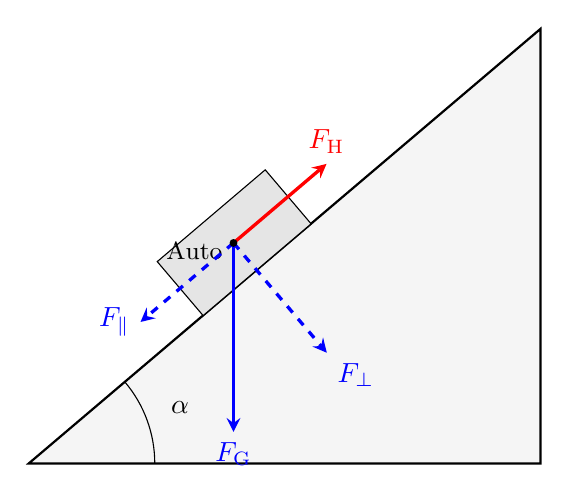
\begin{tikzpicture}[>=stealth]
 \draw[thick, fill=gray!8] (0,0) -- (6.50,0) -- (6.50,5.52) -- cycle;
 \draw (1.6,0) arc (0:40.36:1.6);
 \node at (1.92,0.71) {$\alpha$};
 \begin{scope}[shift={(2.90,2.46)}, rotate=40.36]
  \draw[fill=gray!20] (-0.9,0) rectangle (0.9,0.9);
  \node[font=\small] at (-0.45,0.70) {Auto};
 \end{scope}
 \draw[->, very thick, blue] (2.60,2.80) -- ++(-90.00:2.40) node[anchor=north] {$F_\mathrm{G}$};
 \draw[->, very thick, blue, dashed] (2.60,2.80) -- ++(-49.64:1.83) node[anchor=north west] {$F_\perp$};
 \draw[->, very thick, blue, dashed] (2.60,2.80) -- ++(220.36:1.55) node[anchor=east] {$F_\parallel$};
 \draw[->, very thick, red] (2.60,2.80) -- ++(40.36:1.55) node[anchor=south] {$F_\mathrm{H}$};
 \fill (2.60,2.80) circle (0.05);
\end{tikzpicture}
\end{center}

Wir nehmen an, dass alle Räder gebremst sind (Handbremse und eingelegter Gang). Das Auto bleibt stehen, solange die Haftreibung die Hangabtriebskraft aufbringen kann:
\begin{align}
 m\,g\sin\alpha &\leq \mu_\mathrm{H}\,F_\mathrm{N} = \mu_\mathrm{H}\,m\,g\cos\alpha \quad\Rightarrow\quad \tan\alpha \leq \mu_\mathrm{H}
\end{align}
Für Pneu auf trockener Asphaltstrasse ist $\mu_\mathrm{H} = \muHO$ (FoTaBe S.~189). Der grösste Neigungswinkel ist
\begin{align}
 \alpha &= \wiF = \arctan\left(\muH\right) = \wi \approx \result{\wiP{0}{2}}
\end{align}
Das entspricht einer Steigung von \muHO. Mit der Streuung $\pm\dmuO$ der Haftreibungszahl liegt der Grenzwinkel zwischen $\wiuP{0}{2}$ und $\wioP{0}{2}$.
